\documentclass[]{article}
\usepackage{lmodern}
\usepackage{amssymb,amsmath}
\usepackage{ifxetex,ifluatex}
\usepackage{fixltx2e} % provides \textsubscript
\ifnum 0\ifxetex 1\fi\ifluatex 1\fi=0 % if pdftex
  \usepackage[T1]{fontenc}
  \usepackage[utf8]{inputenc}
\else % if luatex or xelatex
  \ifxetex
    \usepackage{mathspec}
  \else
    \usepackage{fontspec}
  \fi
  \defaultfontfeatures{Ligatures=TeX,Scale=MatchLowercase}
\fi
% use upquote if available, for straight quotes in verbatim environments
\IfFileExists{upquote.sty}{\usepackage{upquote}}{}
% use microtype if available
\IfFileExists{microtype.sty}{%
\usepackage{microtype}
\UseMicrotypeSet[protrusion]{basicmath} % disable protrusion for tt fonts
}{}
\usepackage[margin=1in]{geometry}
\usepackage{hyperref}
\hypersetup{unicode=true,
            pdftitle={STATS 531 Midterm Project},
            pdfauthor={Elliott Evans},
            pdfborder={0 0 0},
            breaklinks=true}
\urlstyle{same}  % don't use monospace font for urls
\usepackage{color}
\usepackage{fancyvrb}
\newcommand{\VerbBar}{|}
\newcommand{\VERB}{\Verb[commandchars=\\\{\}]}
\DefineVerbatimEnvironment{Highlighting}{Verbatim}{commandchars=\\\{\}}
% Add ',fontsize=\small' for more characters per line
\usepackage{framed}
\definecolor{shadecolor}{RGB}{248,248,248}
\newenvironment{Shaded}{\begin{snugshade}}{\end{snugshade}}
\newcommand{\KeywordTok}[1]{\textcolor[rgb]{0.13,0.29,0.53}{\textbf{#1}}}
\newcommand{\DataTypeTok}[1]{\textcolor[rgb]{0.13,0.29,0.53}{#1}}
\newcommand{\DecValTok}[1]{\textcolor[rgb]{0.00,0.00,0.81}{#1}}
\newcommand{\BaseNTok}[1]{\textcolor[rgb]{0.00,0.00,0.81}{#1}}
\newcommand{\FloatTok}[1]{\textcolor[rgb]{0.00,0.00,0.81}{#1}}
\newcommand{\ConstantTok}[1]{\textcolor[rgb]{0.00,0.00,0.00}{#1}}
\newcommand{\CharTok}[1]{\textcolor[rgb]{0.31,0.60,0.02}{#1}}
\newcommand{\SpecialCharTok}[1]{\textcolor[rgb]{0.00,0.00,0.00}{#1}}
\newcommand{\StringTok}[1]{\textcolor[rgb]{0.31,0.60,0.02}{#1}}
\newcommand{\VerbatimStringTok}[1]{\textcolor[rgb]{0.31,0.60,0.02}{#1}}
\newcommand{\SpecialStringTok}[1]{\textcolor[rgb]{0.31,0.60,0.02}{#1}}
\newcommand{\ImportTok}[1]{#1}
\newcommand{\CommentTok}[1]{\textcolor[rgb]{0.56,0.35,0.01}{\textit{#1}}}
\newcommand{\DocumentationTok}[1]{\textcolor[rgb]{0.56,0.35,0.01}{\textbf{\textit{#1}}}}
\newcommand{\AnnotationTok}[1]{\textcolor[rgb]{0.56,0.35,0.01}{\textbf{\textit{#1}}}}
\newcommand{\CommentVarTok}[1]{\textcolor[rgb]{0.56,0.35,0.01}{\textbf{\textit{#1}}}}
\newcommand{\OtherTok}[1]{\textcolor[rgb]{0.56,0.35,0.01}{#1}}
\newcommand{\FunctionTok}[1]{\textcolor[rgb]{0.00,0.00,0.00}{#1}}
\newcommand{\VariableTok}[1]{\textcolor[rgb]{0.00,0.00,0.00}{#1}}
\newcommand{\ControlFlowTok}[1]{\textcolor[rgb]{0.13,0.29,0.53}{\textbf{#1}}}
\newcommand{\OperatorTok}[1]{\textcolor[rgb]{0.81,0.36,0.00}{\textbf{#1}}}
\newcommand{\BuiltInTok}[1]{#1}
\newcommand{\ExtensionTok}[1]{#1}
\newcommand{\PreprocessorTok}[1]{\textcolor[rgb]{0.56,0.35,0.01}{\textit{#1}}}
\newcommand{\AttributeTok}[1]{\textcolor[rgb]{0.77,0.63,0.00}{#1}}
\newcommand{\RegionMarkerTok}[1]{#1}
\newcommand{\InformationTok}[1]{\textcolor[rgb]{0.56,0.35,0.01}{\textbf{\textit{#1}}}}
\newcommand{\WarningTok}[1]{\textcolor[rgb]{0.56,0.35,0.01}{\textbf{\textit{#1}}}}
\newcommand{\AlertTok}[1]{\textcolor[rgb]{0.94,0.16,0.16}{#1}}
\newcommand{\ErrorTok}[1]{\textcolor[rgb]{0.64,0.00,0.00}{\textbf{#1}}}
\newcommand{\NormalTok}[1]{#1}
\usepackage{longtable,booktabs}
\usepackage{graphicx,grffile}
\makeatletter
\def\maxwidth{\ifdim\Gin@nat@width>\linewidth\linewidth\else\Gin@nat@width\fi}
\def\maxheight{\ifdim\Gin@nat@height>\textheight\textheight\else\Gin@nat@height\fi}
\makeatother
% Scale images if necessary, so that they will not overflow the page
% margins by default, and it is still possible to overwrite the defaults
% using explicit options in \includegraphics[width, height, ...]{}
\setkeys{Gin}{width=\maxwidth,height=\maxheight,keepaspectratio}
\IfFileExists{parskip.sty}{%
\usepackage{parskip}
}{% else
\setlength{\parindent}{0pt}
\setlength{\parskip}{6pt plus 2pt minus 1pt}
}
\setlength{\emergencystretch}{3em}  % prevent overfull lines
\providecommand{\tightlist}{%
  \setlength{\itemsep}{0pt}\setlength{\parskip}{0pt}}
%\setcounter{secnumdepth}{0}
\setcounter{section}{1}
% Redefines (sub)paragraphs to behave more like sections
\ifx\paragraph\undefined\else
\let\oldparagraph\paragraph
\renewcommand{\paragraph}[1]{\oldparagraph{#1}\mbox{}}
\fi
\ifx\subparagraph\undefined\else
\let\oldsubparagraph\subparagraph
\renewcommand{\subparagraph}[1]{\oldsubparagraph{#1}\mbox{}}
\fi

%%% Use protect on footnotes to avoid problems with footnotes in titles
\let\rmarkdownfootnote\footnote%
\def\footnote{\protect\rmarkdownfootnote}

%%% Change title format to be more compact
\usepackage{titling}

% Create subtitle command for use in maketitle
\newcommand{\subtitle}[1]{
  \posttitle{
    \begin{center}\large#1\end{center}
    }
}

\setlength{\droptitle}{-2em}
  \title{STATS 531 Midterm Project}
  \pretitle{\vspace{\droptitle}\centering\huge}
  \posttitle{\par}
\subtitle{An Investigation of Democratic Support in the 2018 US Midterm Elections}
  \author{Elliott Evans}
  \preauthor{\centering\large\emph}
  \postauthor{\par}
  \predate{\centering\large\emph}
  \postdate{\par}
  \date{3/7/2018}

\usepackage{amsmath}
\usepackage{amssymb}
\usepackage{amsthm}

\begin{document}
\maketitle

{
\setcounter{tocdepth}{2}
\tableofcontents
}
\newcommand{\DEF}{\overset{\text{def}}{=}}
\newcommand{\PP}{\mathbb{P}}
\newcommand{\RR}{\mathbb{R}}
\newcommand{\ZZ}{\mathbb{Z}}
\newcommand{\EE}{\mathbb{E}}
\newcommand{\IND}{\mathbbm{1}}
\newcommand{\var}{\text{Var}}
\newcommand{\cov}{\text{Cov}}
\newcommand{\logit}{\text{logit}}
\newcommand{\n}{\newline}
\newcommand\loglik{\ell}
\newcommand\R{\mathbb{R}}
\newcommand\data[1]{#1^*}
\newcommand\estimate[1]{\data{#1}}
\newcommand\params{\, ; \,}
\newcommand\transpose{\scriptsize{T}}
\newcommand\eqspace{\quad\quad\quad}
\newcommand\lik{\mathscr{L}}
\newcommand\profileloglik[1]{\ell^\mathrm{profile}_#1}
\newcommand\ar{\phi}
\newcommand\ma{\psi}

\begin{center}\rule{0.5\linewidth}{\linethickness}\end{center}

\subsection{Introduction}\label{introduction}

On Tuesday, November 6, voters in the US will head to the polls to vote
in the \textbf{midterm elections}. Thus, there is an explicit need to
develop a better understanding of what drives the American electorate to
support Republicans or Democrats.

During midterm election years, pollsters love to ask the
``\textbf{generic ballot question}:''

\begin{quote}
``Thinking about the elections in 2018, if the election for U.S.
Congress were held today, would you vote for the Democratic candidate or
the Republican candidate in your district where you live?'' -- Ipsos
2018 Generic Congressional Ballot Question
\end{quote}

The historical results of this question have had an important
association with a party's success in midterm elections. After
controlling for the party in the White House, the generic ballot about
eighteen months before election day is fairly correlated (+0.78) with
the subsequent share of votes cast for the President's party {[}1{]}.

\subsection{Questions of Interest}\label{questions-of-interest}

Due to its importance, we use the generic ballot question to
\textbf{address the following questions}:

\begin{enumerate}
\def\labelenumi{\arabic{enumi}.}
\tightlist
\item
  What kind of time series model is appropriate for modeling Democratic
  support in the 2018 midterms?
\item
  Can we discern any useful information about patterns or cycles with
  regards to Democratic support?
\item
  Is there a relationship between Democratic midterm support and
  President Trump's national approval ratings?
\end{enumerate}

\subsection{Data and Notation}\label{data-and-notation}

To address our questions, we use generic ballot polling {[}2{]} from the
market research company \textbf{Ipsos}, which was given an A-- grade by
FiveThirtyEight's pollster ratings {[}3{]}. Polls are conducted and
issued everyday by Ipsos on a rolling basis, with each poll consisting
of online interviews from Democrats, Republicans, and Independents. Each
poll represents a sample across five days. For our purposes, the date
associated with each poll is the poll's final day of its five-day span.
In our analysis, poll dates range from May 23, 2017 to February 26,
2018.

Generic ballot polls were obtained from FiveThirtyEight's Generic Ballot
Tracker {[}4{]} . To model democratic midterm support, we use the
percentage of voters who responded ``Democrat'' to the generic ballot
question minus the percentage of voters who responded''Republican''
(thus, excluding those voters who claimed they were not voting or were
undecided). Throughout the analysis, we will let the \emph{random}
democratic midterm margin for each time point \(1,2,\dots,N\) be denoted
by \(DEM_1,DEM_2,\dots ,DEM_N\). Similarly, the corresponding observed
values will be \(dem_1,dem_2,\dots ,dem_N\)

The national approval ratings for President Trump are also from Ipsos;
pulled from FiveThirtyEight's presidential approval tracker {[}5{]}. For
our purposes, we focus on his \emph{disapproval} rating (for more direct
comparison to the Democratic midterm margin). Here, we use the
percentage of voters who responded ``disapprove'' to the question of
Donald Trump's performance in office minus the percentage of voters who
responded''approve.'' We will denote his disapproval ratings as
\(TRUMP_1,TRUMP_2,\dots ,TRUMP_N\) with corresponding observed values of
\(trump_1,trump_2,\dots ,trump_N\).

\subsection{Exploratory Analysis}\label{exploratory-analysis}

Here, we perform some exploratory data analysis on the Democratic
midterm polling data (we will use the presidential disapproval ratings
in a later analysis to address our third question). Below, we find the
time series plots for the unaltered and differenced data (i.e.~using
\(dem_i - dem_{i-1}\)). A trend in the unaltered data is difficult to
notice, but the mean appears to decrease from January to March. We also
notice that the time series plot of the differenced data indicates a
possible process that is more ``stable'' then the undifferenced process.
This will be our main motivation for using an \emph{integrated}
autoregressive moving-average model, i.e.~an ARIMA model, in subsequent
analysis. Finally, we observe from the sample autocorrelation plot that
the sample values are fairly correlated for day-lags one to four, and
that the autocorrelation exhibits an oscillatory pattern. Thus, these
data are clearly not independent across time, another motivation for
using an ARIMA model.

\begin{center}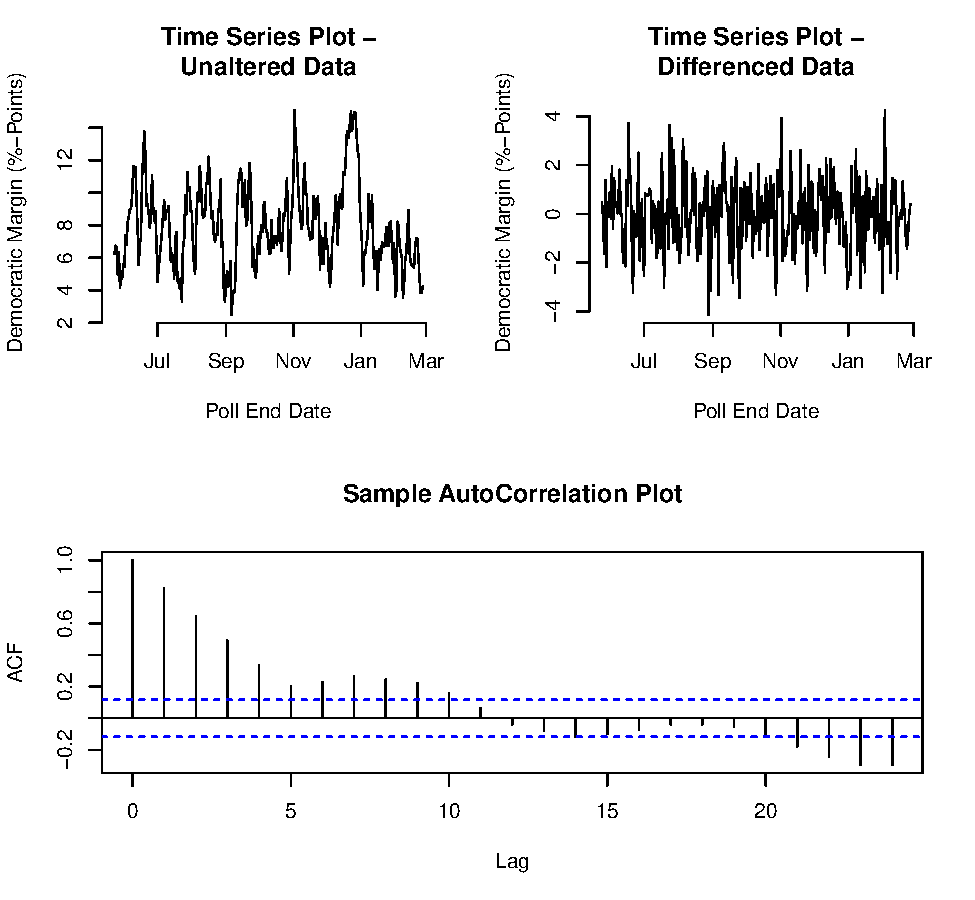
\includegraphics{midterm_project_final_files/figure-latex/eda-1} \end{center}

\subsection{Creating the ARIMA Model}\label{creating-the-arima-model}

\subsubsection{Selection}\label{selection}

We are determined to fit an ARIMA(\(p,1,q\)) model to the democratic
midterm support data and we use AIC as our model selection criteria.
Below we find the AIC values of several ARIMA models with varying
numbers of autoregressive and moving-average terms.

\begin{longtable}[]{@{}lrrrrrr@{}}
\toprule
& MA0 & MA1 & MA2 & MA3 & MA4 & MA5\tabularnewline
\midrule
\endhead
 AR0 & 1008.32 & 1010.32 & 1010.86 & 1008.98 & 1009.99 &
932.61\tabularnewline
 AR1 & 1010.32 & 1012.20 & 991.42 & 997.07 & 979.40 &
934.30\tabularnewline
 AR2 & 1011.03 & 1013.01 & 992.67 & 993.53 & 972.32 &
935.95\tabularnewline
 AR3 & 1013.01 & 1012.56 & 994.32 & 979.39 & 981.39 &
935.98\tabularnewline
 AR4 & 1014.09 & 994.39 & 996.22 & 976.91 & 981.82 &
937.43\tabularnewline
 AR5 & 941.96 & 943.74 & 942.44 & 943.73 & 944.62 &
941.33\tabularnewline
\bottomrule
\end{longtable}

Since we desire to choose an ARIMA model with low AIC value, we find
that ARIMA(\(0,1,5\)) and ARIMA(\(1,1,5\)) should suffice. Because we
desire the Democratic midterm support to be, at least partially, driven
by the previous day's margin, we \textbf{choose to include one
autoregressive term}, i.e.~the \textbf{ARIMA(\(\boldsymbol{1,1,5}\))}
model. Because the difference in AIC values for these models is
relatively small, this should be a sensible decision. Thus, our time
series model for Democratic midterm support is as follows:
\[(1-\phi_1B)(DEM_n-DEM_{n-1} - \mu) = (1+\psi_1B + \psi_2B^2 + \cdots +\psi_5B^5)\epsilon_n \]
where \(\epsilon_1,\epsilon_2,\dots ,\epsilon_N\) are IID Gaussian white
noise terms and \(B\) is the \emph{backshift operator}.

\subsubsection{Fitting}\label{fitting}

We proceed to fit the model above with \(\mu\equiv 0\). The fitted model
output is below.

\begin{Shaded}
\begin{Highlighting}[]
\NormalTok{fit =}\StringTok{ }\KeywordTok{arima}\NormalTok{(genbal_sub}\OperatorTok{$}\NormalTok{dem_margin,}\DataTypeTok{order=}\KeywordTok{c}\NormalTok{(}\DecValTok{1}\NormalTok{,}\DecValTok{1}\NormalTok{,}\DecValTok{5}\NormalTok{),}\DataTypeTok{include.mean=}\NormalTok{T)}
\NormalTok{fit}
\end{Highlighting}
\end{Shaded}

\begin{verbatim}
## 
## Call:
## arima(x = genbal_sub$dem_margin, order = c(1, 1, 5), include.mean = T)
## 
## Coefficients:
##          ar1     ma1      ma2      ma3      ma4      ma5
##       0.0640  -0.099  -0.0433  -0.0557  -0.0899  -0.5974
## s.e.  0.1178   0.105   0.0560   0.0576   0.0587   0.0563
## 
## sigma^2 estimated as 1.588:  log likelihood = -460.15,  aic = 934.3
\end{verbatim}

We find that the root of the AR polynomial is far outside the unit
circle in the complex plane, indicating a \textbf{causal model}:

\begin{verbatim}
## [1] "Roots of the AR Poly: 15.625+0i"
\end{verbatim}

\begin{verbatim}
## [1] "Modulus of the AR Poly: 15.625"
\end{verbatim}

We also find that the roots of the MA polynomial are outside of the
complex unit circle, indicating an \textbf{invertible model}. However,
the roots are far closer than those of the AR polynomial to the boundary
of the unit circle (as seen below). A future analysis may study the
model's potential for invertibility problems.

\begin{verbatim}
## [1] "Roots of the MA Poly: 0.858+0.692i" 
## [2] "Roots of the MA Poly: -0.379+1.048i"
## [3] "Roots of the MA Poly: -0.379-1.048i"
## [4] "Roots of the MA Poly: 0.858-0.692i" 
## [5] "Roots of the MA Poly: -1.109+0i"
\end{verbatim}

\begin{verbatim}
## [1] "Modulus of the MA Poly: 1.102" "Modulus of the MA Poly: 1.114"
## [3] "Modulus of the MA Poly: 1.114" "Modulus of the MA Poly: 1.102"
## [5] "Modulus of the MA Poly: 1.109"
\end{verbatim}

\subsubsection{Diagnostics}\label{diagnostics}

The model diagnostics for the residuals appear to indicate that the
\textbf{residuals are generated from an IID Gaussian white noise
process}. The ACF plot shows most of the autocorrelations falling within
the 95\% confidence bounds, indicating independence across lags, the
QQ-plot shows that the normality assumption on the \(\epsilon_i\) terms
is most likely valid, and the residual v. fitted plot does not hint at
any major heteroskedasticity.

\begin{center}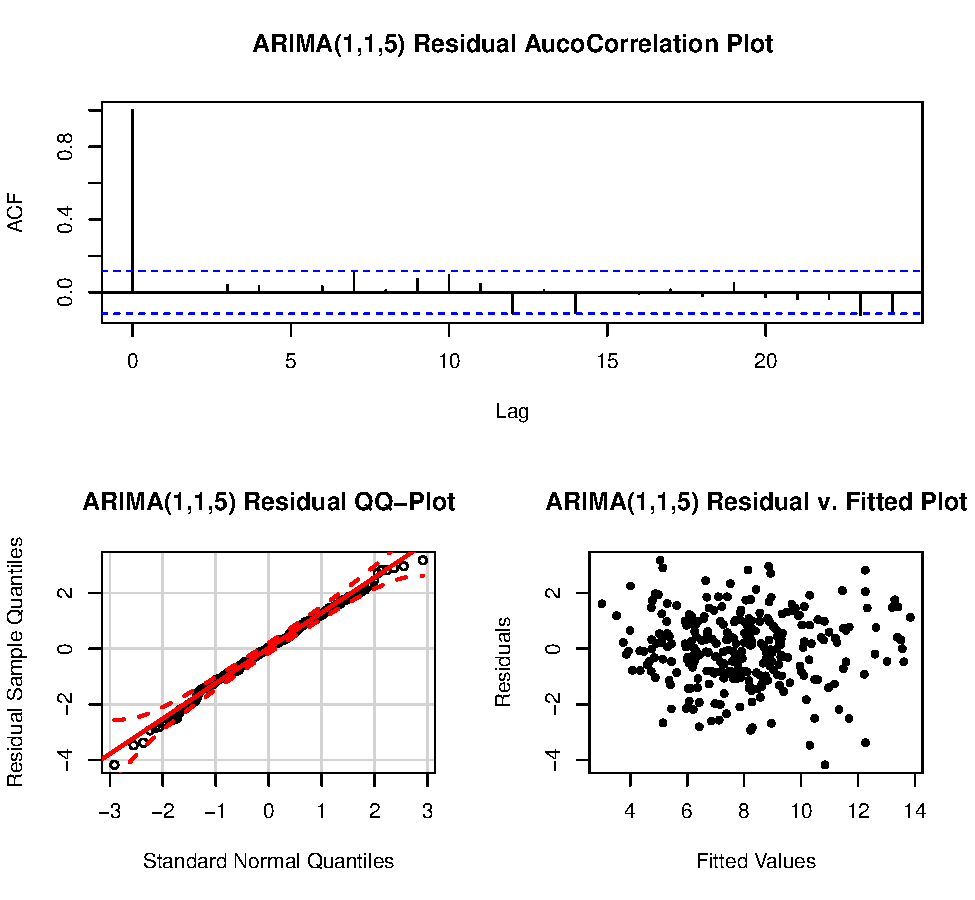
\includegraphics{midterm_project_final_files/figure-latex/diagnostics-1} \end{center}

\subsection{Response to Question One}\label{response-to-question-one}

As our first desire was to generate a model appropriate for the
Democratic midterm support data, we take a moment to explicitly address
this. By choosing an ARIMA time series model with relatively low AIC, we
have generated a model with more predictive power than other comparable
ARIMA models.

Since the model diagnostics have given support to our error terms being
IID Gaussian white noise, it appears that Ipsos generic ballot data can
be sufficiently modeled using an \textbf{ARIMA(1,1,5)} model. We can
view the fitted values below, along with \textbf{Loess smoothing} to
nonparametrically estimate the trend function.

\begin{center}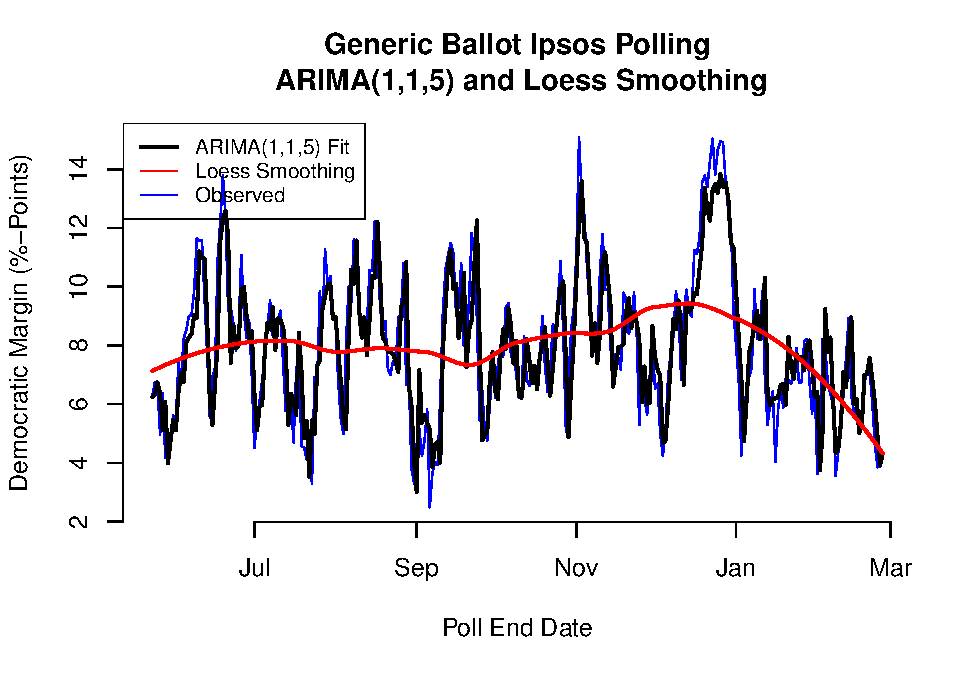
\includegraphics{midterm_project_final_files/figure-latex/fitted-1} \end{center}

We observe that the ARIMA(1,1,5) model appears to fit the data fairly
well. However, using so many moving-average terms might be causing
over-fitting, leading us to believe this is a model better used for
inference than prediction. We also notice that Loess smoothing indicates
that \textbf{mean Democratic support for the midterms potentially
declined from December to the end of February.}

\subsection{Response to Question Two}\label{response-to-question-two}

To answer our second question about useful information regarding cycles
and patterns in our time series, we look again to the generic ballot
data for Democratic midterm support.

We convert the data to its frequency components and observe the
\textbf{unsmoothed and smoothed periodograms}:

\begin{center}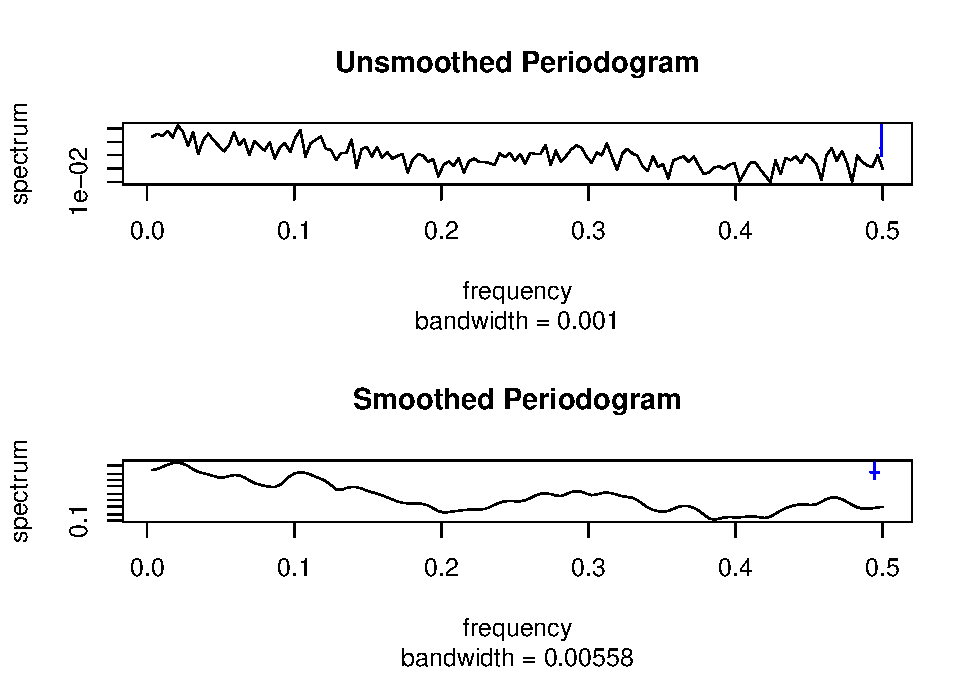
\includegraphics{midterm_project_final_files/figure-latex/periodograms-1} \end{center}

We see that the dominant frequency (from the smoothed periodogram) is
0.104 cycles per day, i.e.~48 days per cycle. However, using the bar in
the upper-right of the periodogram for point-wise 95\% confidence
intervals, we see that this cycle might not be statistically
significant.

A more compelling cycle occurs at frequency 0.104 cycles per day,
i.e.~9.6 days per cycle. We find that using the pointwise confidence
interval for the tip of this peak gives support to the idea that this
peak may not be due to chance variation.

Potential explanations for this dominant cycle of about 10 days could be
(1) the persistence of news stories and/or (2) the importance of
feedback loops in how we perceive support for political parties. In (1),
positive news stories for Democrats may tend to persist for about 10
days, or at least their effects on Democratic midterm support last this
long. In (2), a short-run news story causes a brief negative (or
positive) effect on Democratic support in the polls which, in turn,
becomes a short-run news story itself, creating further losses (or
gains) for Democratic midterm support.

\subsection{The Relationship b/t Midterm Polling and Trump
Disapproval}\label{the-relationship-bt-midterm-polling-and-trump-disapproval}

We suspect that an increase in Democratic support for the midterms might
be driven by an increase in disapproval in President Trump's job
performance. Below, we plot the sample Democratic midterm margins, along
with the sample Trump disapproval margins (and corresponding Loess
smoothing).

\begin{center}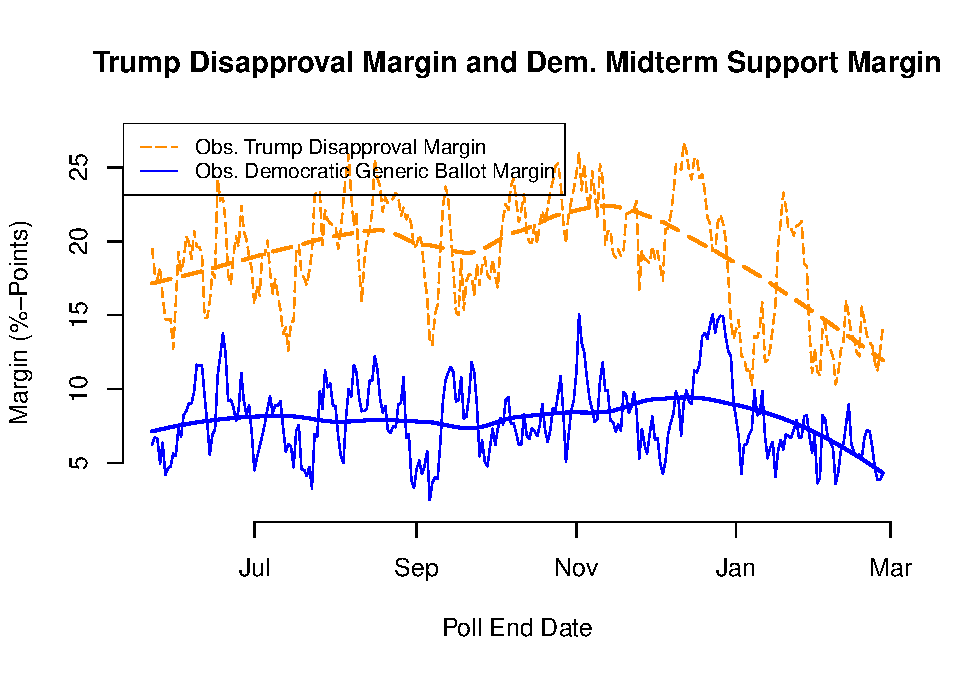
\includegraphics{midterm_project_final_files/figure-latex/trump_v_dem_support-1} \end{center}

We notice that there's a much wider support gap between those who
disapprove/approve of Trump and those who claim to be supporting/not
supporting Democrats in the upcoming midterm elections. This is sensible
since we might expect President Trump to be more polarizing than the
average Democrat or average Republican (which is essentially a matter
for the generic ballot question).

However, we do notice a relationship in the slopes of the estimated
trends across time, with Trump's appearing slightly more extreme for
fixed time intervals. When viewing the scatterplot of Trump's
disapproval margin against Democratic support margin, we do in fact
notice a positive association, however scattered: as Trump becomes more
unpopular, Democratic midterm support on the generic ballot seems to
increase:

\begin{center}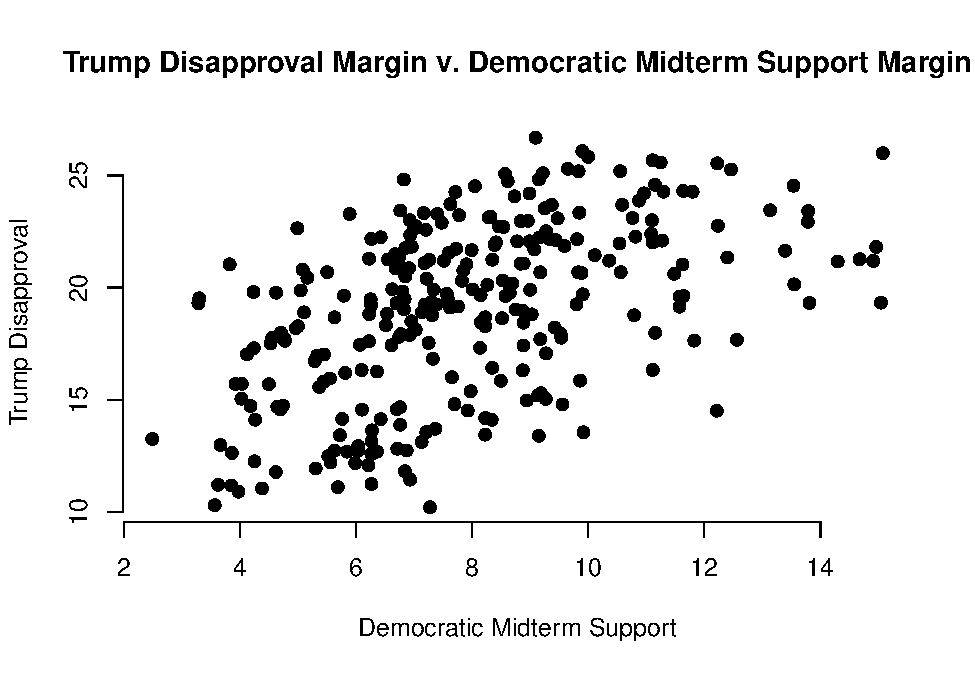
\includegraphics{midterm_project_final_files/figure-latex/scatter-1} \end{center}

Thus, we attempt to regress the Democratic midterm support margin on
Trump's disapproval margin using autocorrelated ARMA errors.

\subsection{Creating the Regression w/ ARMA Errors
Model}\label{creating-the-regression-w-arma-errors-model}

\subsubsection{Selection}\label{selection-1}

First, we run an ordinary regression (i.e.~acting as if the errors of
our model are uncorrelated) and retain the residuals. The results are
below.

\begin{Shaded}
\begin{Highlighting}[]
\NormalTok{fitlinreg =}\StringTok{ }\KeywordTok{lm}\NormalTok{(genbal_sub}\OperatorTok{$}\NormalTok{dem_margin}\OperatorTok{~}\NormalTok{approve_sub}\OperatorTok{$}\NormalTok{dis_margin)}
\KeywordTok{summary}\NormalTok{(fitlinreg)}
\end{Highlighting}
\end{Shaded}

\begin{verbatim}
## 
## Call:
## lm(formula = genbal_sub$dem_margin ~ approve_sub$dis_margin)
## 
## Residuals:
##     Min      1Q  Median      3Q     Max 
## -4.8105 -1.5307 -0.2392  1.2907  6.9975 
## 
## Coefficients:
##                        Estimate Std. Error t value Pr(>|t|)    
## (Intercept)             1.65319    0.65505   2.524   0.0122 *  
## approve_sub$dis_margin  0.33074    0.03372   9.810   <2e-16 ***
## ---
## Signif. codes:  0 '***' 0.001 '**' 0.01 '*' 0.05 '.' 0.1 ' ' 1
## 
## Residual standard error: 2.177 on 277 degrees of freedom
## Multiple R-squared:  0.2578, Adjusted R-squared:  0.2551 
## F-statistic: 96.23 on 1 and 277 DF,  p-value: < 2.2e-16
\end{verbatim}

\begin{Shaded}
\begin{Highlighting}[]
\NormalTok{res =}\StringTok{ }\NormalTok{fitlinreg}\OperatorTok{$}\NormalTok{residuals}
\KeywordTok{acf}\NormalTok{(res,}\DataTypeTok{main=}\StringTok{'AutoCorrelation Plot of Residuals'}\NormalTok{)}
\end{Highlighting}
\end{Shaded}

\begin{center}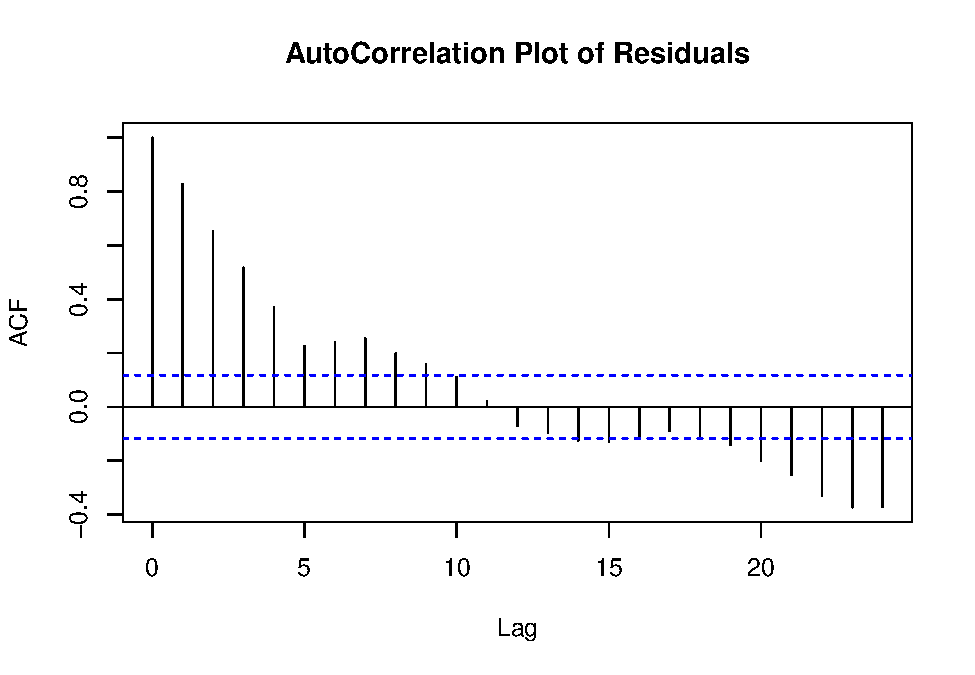
\includegraphics{midterm_project_final_files/figure-latex/linreg-1} \end{center}

From the sample autocorrelation plot above, we see that the residuals of
this linear regression indicate autocorrelated errors, rather than
independent errors. Thus, we identify a proper ARMA model for these
errors. Again, we use AIC as our model selection criteria. Below are the
AIC results for several ARMA(\(p,q\)) models:

\begin{longtable}[]{@{}lrrrrrr@{}}
\toprule
& MA0 & MA1 & MA2 & MA3 & MA4 & MA5\tabularnewline
\midrule
\endhead
 AR0 & 1227.79 & 1039.48 & 942.62 & 949.91 & 847.47 &
848.74\tabularnewline
 AR1 & 905.28 & 904.31 & 906.22 & 900.27 & 848.81 &
848.34\tabularnewline
 AR2 & 904.45 & 906.19 & 908.19 & 895.64 & 850.60 &
850.94\tabularnewline
 AR3 & 906.40 & 908.18 & 882.38 & 884.22 & 848.12 &
847.37\tabularnewline
 AR4 & 904.17 & 908.45 & 878.35 & 882.05 & 847.92 &
849.53\tabularnewline
 AR5 & 903.58 & 888.39 & 863.90 & 862.94 & 849.60 &
851.42\tabularnewline
\bottomrule
\end{longtable}

We see that an \textbf{MA(4) model shold suffice for our model errors},
since this model type provides us with low AIC. Thus, our linear
regression model using a Trump disapproval covariate and MA(4) errors is
as follows:

\begin{align*}
DEM_i &= \beta_0 +  \beta_1TRUMP_i + \epsilon_i,\qquad i=1,2,\dots ,N\\
\epsilon_i &= w_i + \psi_1w_{i-1} + \psi_2 w_{i-2} + \psi_3 w_{i-3} + \psi_4 w_{i-4}\\
w_i &\sim IID\, N(0,\sigma^2).
\end{align*}

\subsubsection{Fitting}\label{fitting-1}

The results of fitting the linear regression with MA(4) errors is below:

\begin{Shaded}
\begin{Highlighting}[]
\NormalTok{fitreg =}\StringTok{ }\KeywordTok{arima}\NormalTok{(genbal_sub}\OperatorTok{$}\NormalTok{dem_margin,}\DataTypeTok{order=}\KeywordTok{c}\NormalTok{(}\DecValTok{0}\NormalTok{,}\DecValTok{0}\NormalTok{,}\DecValTok{4}\NormalTok{),}
            \DataTypeTok{xreg =} \KeywordTok{cbind}\NormalTok{(}\DataTypeTok{TRUMPDISAPPROVAL =}\NormalTok{ approve_sub}\OperatorTok{$}\NormalTok{dis_margin))}
\KeywordTok{summary}\NormalTok{(fitreg)}
\end{Highlighting}
\end{Shaded}

\begin{verbatim}
## 
## Call:
## arima(x = genbal_sub$dem_margin, order = c(0, 0, 4), xreg = cbind(TRUMPDISAPPROVAL = approve_sub$dis_margin))
## 
## Coefficients:
##          ma1     ma2     ma3     ma4  intercept  TRUMPDISAPPROVAL
##       0.9742  0.8851  0.7336  0.6379     0.0654            0.4127
## s.e.  0.0448  0.0647  0.0662  0.0460     0.8107            0.0402
## 
## sigma^2 estimated as 1.14:  log likelihood = -415.68,  aic = 845.35
## 
## Training set error measures:
##                       ME     RMSE       MAE       MPE     MAPE     MASE
## Training set 0.005843376 1.067931 0.8362786 -2.328961 11.74584 0.721483
##                    ACF1
## Training set 0.03406737
\end{verbatim}

\begin{Shaded}
\begin{Highlighting}[]
\NormalTok{fitreg_detrended =}\StringTok{ }\KeywordTok{arima}\NormalTok{(genbal_sub}\OperatorTok{$}\NormalTok{dem_margin,}\DataTypeTok{order=}\KeywordTok{c}\NormalTok{(}\DecValTok{0}\NormalTok{,}\DecValTok{0}\NormalTok{,}\DecValTok{4}\NormalTok{))}
\NormalTok{chi_sq_stat =}\StringTok{ }\DecValTok{2}\OperatorTok{*}\NormalTok{(fitreg}\OperatorTok{$}\NormalTok{loglik }\OperatorTok{-}\StringTok{ }\NormalTok{fitreg_detrended}\OperatorTok{$}\NormalTok{loglik)}
\NormalTok{chi_sq_stat}
\end{Highlighting}
\end{Shaded}

\begin{verbatim}
## [1] 89.18129
\end{verbatim}

\begin{Shaded}
\begin{Highlighting}[]
\KeywordTok{qchisq}\NormalTok{(.}\DecValTok{95}\NormalTok{,}\DecValTok{1}\NormalTok{,}\DataTypeTok{lower.tail=}\NormalTok{T)}
\end{Highlighting}
\end{Shaded}

\begin{verbatim}
## [1] 3.841459
\end{verbatim}

We observe that, due to the relatively small standard errors, 95\%
confidence intervals for our moving-average parameters \emph{and}
regression parameter indicate statistically significant differences from
zero. In addition, in comparing this model to the detrended version
without the Trump disapproval covariate, we find evidence that the Trump
disapproval regression parameter is significant. In performing the
likelihood ratio test of \(H_0: \beta_1=0\) against
\(H_a:\beta_1\neq 0\), we obtain a chi-square statistic of 89.2, far
more extreme than \(\chi^2_{0.95,1}=3.84\). Thus, we \textbf{reject the
null model in favor of the regression model that includes Donald Trump's
disapproval margin} as an explainer of the Democratic midterm support
margin.

While we omit the diagnostics for this model, we note that investigation
of the sample autocorrelation plot, QQ-plot, and residual v. fitted
plot, all indicate that an \textbf{IID Gaussian white noise process for
\(\boldsymbol{w_1,w_2,\dots,w_N}\) is appropriate}.

\subsection{Response to Question Three}\label{response-to-question-three}

Here, we tackle our final question of interest. There does, indeed,
appear to be a relationship between Donald Trump's national disapproval
rating and Democratic midterm support on the generic ballot. From the
section above, we noted that a likelihood-ratio test rejects the null
detrended model in favor of the model that uses Trump's disapproval
ratings as a model covariate.

Our model estimates \(\hat{\beta_1} = +0.4127\). Thus, as Donald Trump's
disapproval margin increases, we expect the Democratic support margin
for the midterms to increase. To visually assess the validity of this
model, we present the observed and model-fitted values below:

\begin{center}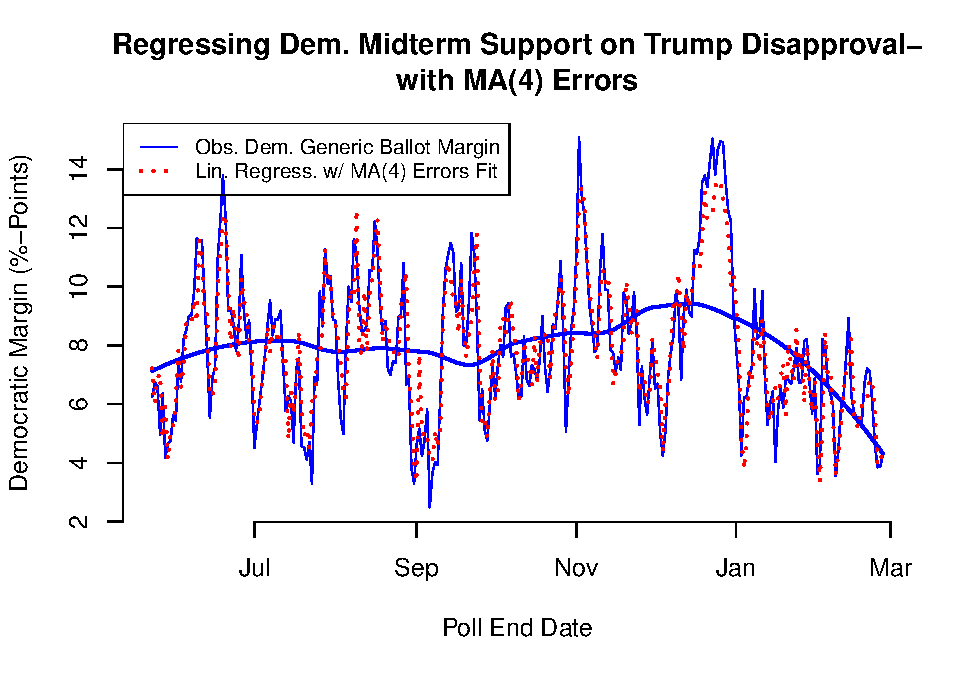
\includegraphics{midterm_project_final_files/figure-latex/linreg_arma_errors_fit-1} \end{center}

We observe that the regression model with MA(4) errors appears to fit
the data well and can safely be used for inference. Thus, we find
reasonable evidence for Trump's disapproval being an explainer of the
variation in Democratic midterm support.

\subsection{Conclusions}\label{conclusions}

We set out to answer three questions, as noted in section 2. Here, we
summarize our results succinctly:

\begin{enumerate}
\def\labelenumi{\arabic{enumi}.}
\item
  An ARIMA(1,1,5) model appears to model the Ipsos generic ballot
  Democratic midterm support margin quite well. However, further
  analysis may be performed to assess the validity of a more simple
  ARIMA(0,1,5) model.
\item
  We find that a dominant cycle in Democratic midterm support is around
  10 days. This could be due to effects of persisting news cycles in the
  media that either benefit or harm the image of national Democrats.
\item
  We do, in fact, find a relationship between Trump's disapproval and
  generic ballot Democratic support. Using a linear regression model
  with MA(4) errors, we found that increased Trump disapproval appears
  to result in increased Democratic support for the midterm elections.
\end{enumerate}

\subsection{References}\label{references}

{[}1{]} Enten, Harry. ``Here's The Best Tool We Have For Understanding
How The Midterms Are Shaping Up.'' FiveThirtyEight, FiveThirtyEight, 5
June 2017,
\url{fivethirtyeight.com/features/heres-the-best-tool-we-have-for-understanding-how-the-midterms-are-shaping-up/}.

{[}2{]} Ipsos Public Affairs. Core Political Data, 2018,
\url{www.ipsos.com/sites/default/files/ct/news/documents/2018-02/2018_reuters_tracking_-_core_political_02_28_2018.pdf}.

{[}3{]} Silver, Nate. ``FiveThirtyEight's Pollster Ratings.''
FiveThirtyEight, 5 Aug. 2016,
\url{projects.fivethirtyeight.com/pollster-ratings/}.

{[}4{]} Silver, Nate. ``Are Democrats Or Republicans Winning The Race
For Congress?'' FiveThirtyEight, 2 Mar. 2018,
\url{projects.fivethirtyeight.com/congress-generic-ballot-polls/?ex_cid=rrpromo}.

{[}5{]} Silver, Nate. ``How Popular Is Donald Trump?'' FiveThirtyEight,
2 Mar. 2018,
\url{projects.fivethirtyeight.com/trump-approval-ratings/?ex_cid=rrpromo}.


\end{document}
